% Local, Open-Weight Agentic Coding
% Copyright (c) 2026 Thomas Ascher
% SPDX-License-Identifier: CC-BY-4.0
% Compile with: lualatex local_agentic_coding.tex
\documentclass[aspectratio=169,10pt]{beamer}

\usepackage{fontspec}
\usepackage{xcolor}
\usepackage{graphicx}
\usepackage{tabularx}
\usepackage{array}
\usepackage{booktabs}
\usepackage{hyperref}

\setmainfont{Noto Sans}
\setsansfont{Noto Sans}
\setmonofont{Noto Sans Mono}
\renewcommand{\familydefault}{\sfdefault}

% ---------- palette: conservative corporate, light background ----------
\definecolor{bg}{HTML}{FFFFFF}
\definecolor{bgraised}{HTML}{F2F4F7}
\definecolor{fg}{HTML}{1B1F26}
\definecolor{muted}{HTML}{5B6472}
\definecolor{accent}{HTML}{1F4E79}
\definecolor{accent2}{HTML}{96702E}
\definecolor{good}{HTML}{1E6B3C}
\definecolor{bad}{HTML}{9B2226}
\definecolor{line}{HTML}{C9CFD8}

% ---------- theme skeleton (no external theme, hand-built) ----------
\usetheme{default}
\setbeamertemplate{navigation symbols}{}
\beamertemplatenavigationsymbolsempty

\setbeamercolor{background canvas}{bg=bg}
\setbeamercolor{normal text}{fg=fg,bg=bg}
\setbeamercolor{structure}{fg=accent}
\setbeamercolor{title}{fg=fg}
\setbeamercolor{frametitle}{fg=fg,bg=bg}
\setbeamercolor{section in toc}{fg=fg}
\setbeamercolor{itemize item}{fg=accent}
\setbeamercolor{itemize subitem}{fg=accent2}
\setbeamercolor{block title}{fg=bg,bg=accent}
\setbeamercolor{block body}{fg=fg,bg=bgraised}
\setbeamercolor{footline}{fg=muted,bg=bg}
\setbeamercolor{caption name}{fg=muted}

\setbeamerfont{frametitle}{series=\bfseries,size=\Large}
\setbeamerfont{footline}{size=\tiny}
\setbeamertemplate{itemize items}[circle]
\setbeamertemplate{blocks}[rounded]

\setbeamertemplate{frametitle}{
  \vspace{0.4em}
  {\displayfont\usebeamercolor[fg]{frametitle}\usebeamerfont{frametitle}\insertframetitle}
  \par
  \vspace{-0.35em}
  {\color{accent}\rule{\linewidth}{1.1pt}}
}

\setbeamertemplate{footline}{}

\title{\textcolor{fg}{Local, Open-Weight Agentic Coding}}
\author{\textcolor{fg}{Thomas Ascher}}
\date{\textcolor{muted}{August 31, 2026}}

% helper: small source citation line
\newcommand{\srcline}[1]{{\scriptsize\color{muted} Source: #1}}
% helper: plain bold status word (color param kept for call-site compatibility,
% intentionally unused -- reads plainer without it)
\newcommand{\statustag}[2]{\textbf{#2}}

\newfontfamily\displayfont{Noto Sans Display}

\begin{document}

\begin{frame}[plain]
  \vfill
  \begin{center}
    {\displayfont\usebeamercolor[fg]{title}\Huge\textbf{Local, Open-Weight}}\\[0.2em]
    {\displayfont\usebeamercolor[fg]{title}\Huge\textbf{Agentic \textcolor{accent}{Coding}}}\\[1.2em]
    {\small\color{bad}\textbf{Personal research --- not evaluated or
    approved for company use}}\\[1.2em]
    {\color{fg}\textbf{Thomas Ascher}}\\
    {\small\color{muted}August 31, 2026}\\[0.8em]
    {\scriptsize\color{muted}\href{https://creativecommons.org/licenses/by/4.0/}{CC BY 4.0}}
  \end{center}
  \vfill
\end{frame}

\begin{frame}{Agentic coding, open-weight models}
  \begin{itemize}
    \item \textbf{Agentic} --- a coding harness loops the model, which runs
      on an inference server (act, observe the result, decide the next
      step, repeat) instead of giving one answer and stopping
    \item \textbf{Open-weight} --- the model itself is downloadable and
      runs on your own hardware, not accessed only through someone else's
      API
    \item \textbf{The risk} --- many agentic tools run unsandboxed, doing
      whatever your account can already do without elevation: depending on
      settings, that can mean modifying or deleting files, installing
      software, or reaching the network without confirmation
  \end{itemize}
\end{frame}

\section{Why Local}

\begin{frame}{For and against}
  \begin{columns}[T]
    \begin{column}{0.5\textwidth}
      \centering\textbf{\textcolor{good}{For}}\par\vspace{0.4em}
      \begin{itemize}
        \small
        \item \textbf{Data sovereignty} --- code and secrets never leave the
          premises
        \item \textbf{No per-token cost} --- hardware is a one-time
          investment
        \item \textbf{Offline capability} --- independent of vendor uptime
          or rate limits
        \item \textbf{Full control} --- pin a version, fine-tune as needed
      \end{itemize}
    \end{column}
    \begin{column}{0.5\textwidth}
      \centering\textbf{\textcolor{bad}{Against}}\par\vspace{0.4em}
      \begin{itemize}
        \small
        \item \textbf{Lower ceiling} --- a meaningful gap to frontier models
          on demanding tasks
        \item \textbf{Lower throughput} --- trails a hosted API; setup and
          maintenance become your responsibility
        \item \textbf{Open tooling lags} --- first-party options exist for
          both IDE and CLI, but open alternatives trail their polish
      \end{itemize}
    \end{column}
  \end{columns}
\end{frame}

\begin{frame}{Edge model vs.\ frontier model}
  \footnotesize
  \renewcommand{\arraystretch}{1.08}
  \begin{center}
  \begin{tabular}{l l l}
    \toprule
    & \textbf{Qwen3.6-35B-A3B} & \textbf{Qwen3.8-Max} \\
    \midrule
    Total / active parameters & 35B / 3B & 2.4T / 95B \\
    Architecture & Mixture-of-Experts & Mixture-of-Experts \\
    Experts & 256 (8 routed + 1 shared) & 512 (10 routed + 1 shared) \\
    Context window & 262K & 1M \\
    \midrule
    Terminal-Bench & 52.5\% & 86.6\% \\
    \bottomrule
  \end{tabular}
  \end{center}
  \vspace{0.5em}
  \textbf{\textcolor{accent}{\textasciitilde{}69x}} fewer total parameters,
  \textbf{\textcolor{accent}{\textasciitilde{}32x}} fewer active, with a
  \textbf{34-point} gap on one of the standard benchmarks --- yet the edge
  model still delivers functional software.
  \vspace{0.4em}\\
  \color{muted} Mixture-of-Experts: each expert is a specialized
  sub-network --- a router activates only a few per token, unlike a dense
  model where every parameter fires every time. Far less
  compute-intensive, but generally harder to fine-tune.
\end{frame}

\begin{frame}{Good enough for the task}
  \begin{block}{Microsoft's strategy}
    \small Route routine work to \textbf{compact specialist models}, and
    reserve \textbf{frontier models} for the cases specialists cannot
    handle.
  \end{block}
  \vspace{0.5em}
  \begin{itemize}
    \item MAI-Cyber-1-Flash tops its benchmark at half a frontier model's
      cost, escalating only genuinely hard cases.
  \end{itemize}
\end{frame}

\section{Hardware}

\begin{frame}{Hardware: what actually matters}
  \begin{itemize}
    \item \textbf{VRAM beats raw compute} --- a model that overflows VRAM
      loses performance; more memory outperforms more speed.
    \item \textbf{\textcolor{accent}{12\,GB VRAM is the practical floor}} --- for
      running models capable of agentic coding.
    \item \textbf{Unified memory trades speed for capacity} --- the
      architecture behind integrated GPUs; it runs at a fraction of a
      discrete GPU's throughput.
    \item \textbf{NPUs are not an option} --- software support remains
      immature, and a discrete GPU outperforms them well before reaching a
      coding-capable model size.
    \item \textbf{Custom accelerators are mainly for renting} --- TPU
      (Google), Trainium (AWS), Maia (Microsoft): all cloud-rented, none
      sold for a desktop.
    \item \textbf{On the horizon} --- NVIDIA is developing direct GPU-to-SSD
      access to extend memory capacity.
  \end{itemize}
\end{frame}

\begin{frame}{Hardware: NVIDIA vs.\ AMD and Intel}
  \begin{itemize}
    \item \textbf{NVIDIA}
      \begin{itemize}
        \item Budget --- RTX 5060 Ti, 16\,GB, \textasciitilde{}€600--700
        \item Top of the line (consumer) --- RTX 5090, 32\,GB,
          \textasciitilde{}€3{,}000+
        \item More options exist above this, but they target enterprise
          buyers.
      \end{itemize}
    \item \textbf{AMD and Intel} --- offer more memory capacity for less, but
      software support lags NVIDIA's ecosystem.
  \end{itemize}
\end{frame}

\section{Tooling}

\begin{frame}{Tooling: the inference server}
  An OpenAI-compatible API is required by most coding harnesses --- LiteLLM
  provides that layer when a server does not speak it natively.
  \vspace{0.6em}

  \textbf{OpenAI-compatible API providers:}
  \vspace{0.3em}
  \begin{columns}[T]
    \begin{column}{0.48\textwidth}
      \centering\textbf{Simple}\par\vspace{0.4em}
      \begin{itemize}
        \small
        \item \textbf{Ollama} --- easiest way to get started
        \item \textbf{llama.cpp} --- the inference core Ollama wraps
      \end{itemize}
    \end{column}
    \begin{column}{0.48\textwidth}
      \centering\textbf{Advanced}\par\vspace{0.4em}
      \begin{itemize}
        \small
        \item \textbf{vLLM} --- the default choice; reuses an exact shared
          prefix (e.g.\ a fixed system prompt) when enabled
        \item \textbf{SGLang} --- reuses shared context automatically, even
          as it branches, better suited to a coding agent's changing files
      \end{itemize}
    \end{column}
  \end{columns}
\end{frame}

\begin{frame}{Tooling: the coding harness}
  \begin{columns}[T]
    \begin{column}{0.48\textwidth}
      \centering\textbf{VS Code Integration}\par\vspace{0.4em}
      \begin{itemize}
        \small
        \item \textbf{Cline} --- autonomous VS Code extension, built for
          hands-off file edits and terminal execution
        \item \textbf{GitHub Copilot Chat + Ollama connector} --- native
          Copilot integration, built for zero-friction team adoption
      \end{itemize}
    \end{column}
    \begin{column}{0.48\textwidth}
      \centering\textbf{Standalone}\par\vspace{0.4em}
      \begin{itemize}
        \small
        \item \textbf{opencode} --- provider-agnostic CLI, TUI or web UI,
          built for scripting and automation
        \item \textbf{OpenHands} --- sandboxed agent built for production
          automation and benchmarking
        \item \textbf{GitHub Copilot CLI} --- Microsoft's own terminal
          agent, built for teams already standardized on Copilot
      \end{itemize}
    \end{column}
  \end{columns}
  \vspace{0.8em}
  \small\color{muted} Not every available open-source tool prioritizes local
  models --- some monetize via a hosted subscription, treating any local
  server as a secondary path.
\end{frame}

\begin{frame}{Tooling: opencode}
  \centering
  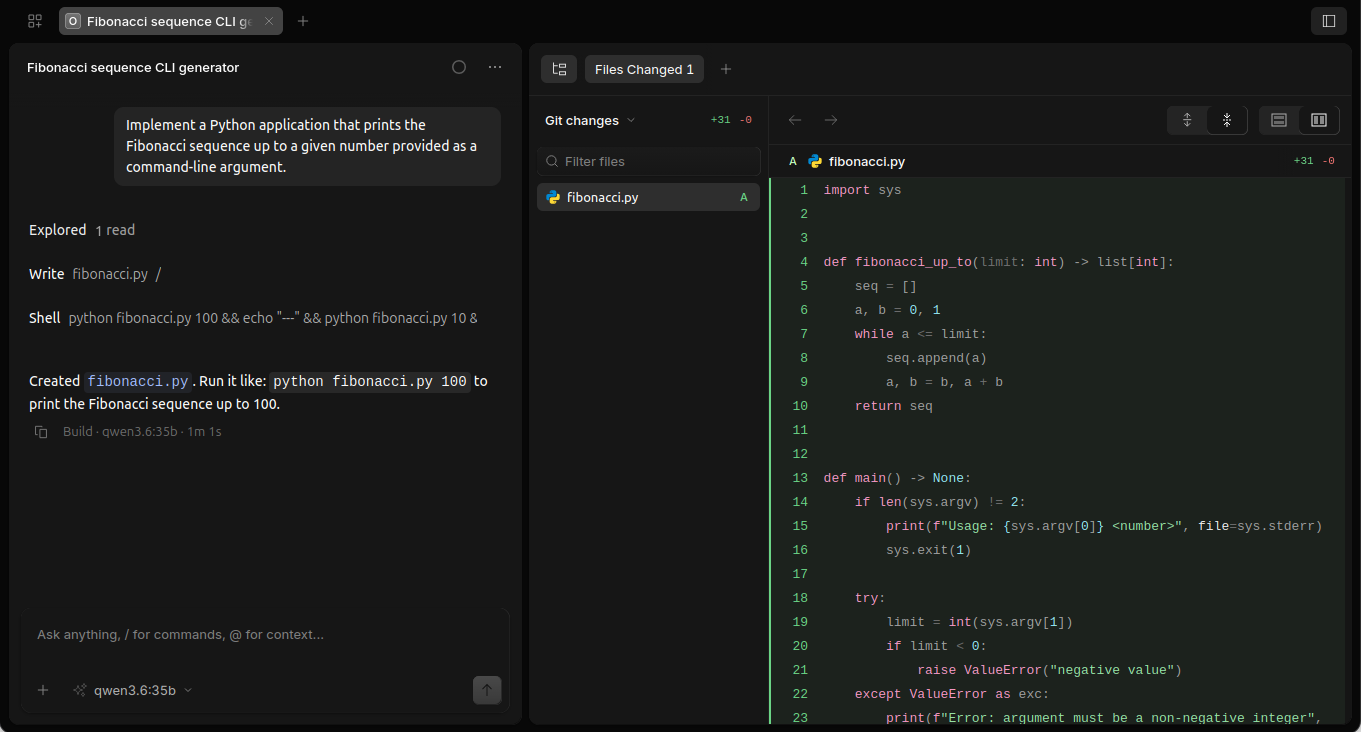
\includegraphics[height=0.78\textheight,keepaspectratio]{opencode.png}
\end{frame}

\section{Picking a Model}

\begin{frame}{Model sources and requirements}
  \begin{columns}[T]
    \begin{column}{0.48\textwidth}
      \centering\textbf{Sources}\par\vspace{0.4em}
      \begin{itemize}
        \small
        \item \textbf{Hugging Face} --- raw weights, every quantization
          variant, full model card
        \item \textbf{Ollama's library} --- pre-quantized, one-command pulls
      \end{itemize}
    \end{column}
    \begin{column}{0.48\textwidth}
      \centering\textbf{Requirements}\par\vspace{0.4em}
      \begin{itemize}
        \footnotesize
        \item \textbf{\textcolor{accent}{20B--70B parameters}} --- below
          20B, models routinely struggle with agentic coding regardless of
          architecture; above \textasciitilde{}70B Mixture-of-Experts
          (MoE) stops fitting consumer hardware
        \item \textbf{Dense} should fit entirely in VRAM or performance
          suffers; \textbf{MoE} should fit entirely in system RAM (only
          active experts need to be VRAM-fast)
        \item \textbf{Q4 quantization} --- the realistic ceiling on a
          consumer card
        \item \textbf{32K minimum context} --- needed to hold a session's
          files and tool output
        \item \textbf{Tool calling support} --- required by every agentic
          tool here; streaming is common but not universal
      \end{itemize}
    \end{column}
  \end{columns}
\end{frame}

\section{Benchmarks}

\begin{frame}{Benchmarks: no single standard}
  \begin{itemize}
    \small
    \item \textbf{Many benchmarks, little overlap} --- LiveCodeBench and
      Terminal-Bench are just two of dozens, each measuring something
      different
    \item \textbf{Static vs.\ agentic} --- one finished answer versus many
      steps through a coding harness; a model can lead on one and trail on
      the other
    \item \textbf{Meta-benchmark tools help} --- tools like
      \texttt{inspect\_evals} bundle many of them behind one runner
    \item \textbf{Setup is a real barrier} --- high system requirements,
      complex setup, and runs are slow and costly to scale
    \item \textbf{Reporting is inconsistent} --- open-weight models get
      thinner coverage, and numbers are often not comparable across sources
  \end{itemize}
\end{frame}

\begin{frame}{Recommended models}
  \footnotesize
  \renewcommand{\arraystretch}{1.2}
  \begin{center}
  \begin{tabular}{l l l l}
    \toprule
    \textbf{Model (total/active)} & \textbf{LiveCodeBench} & \textbf{Terminal-Bench} & \textbf{License} \\
    \midrule
    gemma4:26b (26B/4B) & 77.1\% & --- & Apache 2.0 \\
    laguna-xs-2.1:latest (33B/3B) & --- & 37.5\% & OpenMDW-1.1 \\
    qwen3.6:35b (35B/3B) & 80.4\% & 52.5\% & Apache 2.0 \\
    ornith-1.5:35b (35B/3B) & \textasciitilde{}85\%* & 67.8\% & MIT \\
    nemotron-3.5-lightning:30b (30B/3B) & --- & 24.6\% & OpenMDW-1.1 \\
    \bottomrule
  \end{tabular}
  \end{center}
  \vspace{0.4em}
  \footnotesize *Reported as a combined LiveCodeBench/HumanEval figure, not an
  isolated LiveCodeBench score --- treat as approximate.\\[0.3em]
  \color{muted} nemotron-3.5-lightning's Terminal-Bench score is the
  weakest here, but across my own full agentic coding sessions it never
  once stopped early declaring itself done while leaving broken software
  behind --- every other model in this table did, at least once.
  Stability, not peak score, is its case.
\end{frame}

\begin{frame}{Key takeaways}
  \begin{itemize}
    \item As outlined at the start, the trade-off remains: a lower ceiling
      and slower throughput than a hosted API, with open-source tooling
      trailing commercial polish --- in exchange for data control, cost
      predictability, and independence.
    \item A 20B+, open-weight, tool-calling model on a single consumer GPU
      can deliver working software today, not just a future promise.
    \item Within that range, more parameters generally means more
      capability, and MoE gets there without the full compute cost of a
      dense model the same size.
    \item Consistency, not only peak score, is what actually separates
      these models in practice --- evaluate performance across attempts,
      not just the best result.
    \item Setup can be straightforward: install Ollama, pull a model, and
      point a coding harness at it.
  \end{itemize}
\end{frame}

\appendix
\section{Appendix: Setup Reference}

\begin{frame}{Setting up: Ollama}
  \begin{itemize}
    \item \textbf{Install}
      \begin{itemize}
        \item Linux --- \texttt{curl -fsSL ollama.com/install.sh \textbar\ sh}
        \item Windows --- \texttt{winget install -{}-id Ollama.Ollama}
      \end{itemize}
    \item \textbf{Pull a model} --- \texttt{ollama pull qwen3.6:35b}
    \item \textbf{Set the context window} --- environment variable
      \texttt{OLLAMA\_CONTEXT\_LENGTH=65536}, a fallback for clients that do
      not set their own (on Windows, also settable in the Ollama GUI)
      \begin{itemize}
        \item \textbf{32K} is the recommended minimum for agentic coding
        \item \textbf{64K or higher} is safer for longer sessions, but
          depends on available VRAM
      \end{itemize}
    \item \textbf{Default API URL} --- \texttt{http://localhost:11434/v1}
  \end{itemize}
\end{frame}

\begin{frame}{Setting up: GitHub Copilot Chat}
  \begin{itemize}
    \small
    \item Install the latest VS Code --- no subscription is required.
    \item In GitHub Copilot Chat's model picker, open the gear icon sitting
      inside
      the models list, then use \textbf{Install Model Providers} ---
      select \textbf{Ollama} from the list of extensions and click
      \textbf{Install}.
    \item Select the specific model (e.g.\ \texttt{qwen3.6:35b}) from
      \textbf{Other Models} in the model list.
  \end{itemize}
\end{frame}

\begin{frame}[fragile]{Setting up: opencode}
  \begin{columns}[T]
    \begin{column}{0.46\textwidth}
      \footnotesize
      \begin{itemize}
        \item \textbf{Install}
          \begin{itemize}
            \item Linux --- \texttt{curl -fsSL\\opencode.ai/install \textbar\ bash}
            \item Windows --- \texttt{winget install\\-{}-id SST.opencode}
          \end{itemize}
        \item \textbf{Add Ollama as a provider} in \texttt{opencode.jsonc}
          (right)
          \begin{itemize}
            \item Linux --- \texttt{\char`\~/.config/opencode/}
            \item Windows --- \texttt{\scriptsize\%USERPROFILE\%\textbackslash.config\textbackslash\\opencode\textbackslash}
          \end{itemize}
        \item \textbf{Run it} --- \texttt{opencode} (or \texttt{opencode
          web}), then select \texttt{qwen3.6:35b} from the model list
      \end{itemize}
    \end{column}
    \begin{column}{0.54\textwidth}
      \footnotesize
      \begin{verbatim}
{
  "$schema":
    "https://opencode.ai/config.json",
  "provider": {
    "ollama": {
      "npm": "@ai-sdk/openai-compatible",
      "name": "Ollama",
      "options": {
        "baseURL":
          "http://localhost:11434/v1"
      },
      "models": {
        "qwen3.6:35b": {
          "name": "qwen3.6:35b"
        }
      }
    }
  }
}
      \end{verbatim}
    \end{column}
  \end{columns}
\end{frame}

\begin{frame}[fragile]{Setting up: GitHub Copilot CLI}
  \begin{itemize}
    \item \textbf{Install}
      \begin{itemize}
        \item Linux --- \texttt{curl -fsSL gh.io/copilot-install \textbar\ bash}
        \item Windows --- \texttt{winget install -{}-id GitHub.Copilot}
      \end{itemize}
    \item \textbf{Configure Ollama as the provider} --- environment
      variables:
      \begin{itemize}
        \item \texttt{COPILOT\_PROVIDER\_BASE\_URL=http://localhost:11434/v1}
        \item \texttt{COPILOT\_MODEL=qwen3.6:35b}
      \end{itemize}
  \end{itemize}
\end{frame}

\end{document}
